Two main sources of SM background can be distinguished in this analysis. 
The first category is the reducible or detector background which includes 
events containing electrons with mis-measured charge, mainly from the production of top quark pairs, and events 
containing at least one non-prompt or fake lepton (FNP), which mainly originate from hadron decays in events containing 
top quarks, $W$ or $Z$ bosons. Data-driven methods used for the estimation
of this background are described in Section~\ref{sec:DD_bkg}. The second category consists of events 
with two same-sign prompt leptons or at least three prompt leptons and is 
estimated using the MC samples described in Section~\ref{sec:dataMC}. 
Since diboson and $\ttbar V$ events are the main backgrounds in the signal regions, 
dedicated validation regions (VR) with an enhanced contribution from these processes 
are defined to verify the background predictions from the simulation (see Section~\ref{sec:valid}).


\subsection{Detector background estimation methods} 
\label{sec:DD_bkg}

Background events due to charge mis-identification concerns only the electron. The probability of mis-identifying the 
charge of a muon is checked in both data and MC simulation, and found to be negligible in the kinematic range relevant to this analysis.
The contribution of charge-flip events to the SR/VR yields is estimated using the data. 
The electron charge-flip probability is extracted in a $Z/\gamma^{*}\to ee$ data sample using a likelihood fit 
which takes as input the numbers of same-sign and opposite-sign electron pairs observed in a window around the $Z$ mass. 
The charge-flip probability is a free parameter of the fit and is extracted as a function of the electron $\pt$ and $\eta$. 
These probabilities are in the range \textcolor{red}{UPDATE:1--5\%} and \textcolor{red}{UPDATE:0.1--1\%} for the candidate 
and signal electrons respectively.
The event yield of this background in the signal or validation regions is obtained by applying the measured charge-flip probability 
to the data regions with the same kinematic requirements as the signal or validation regions but with opposite-sign lepton pairs. 

The contribution from fake or non-prompt leptons (such as hadrons mis-identified as leptons, 
leptons originating from heavy-flavour decays, and electrons from photon conversions) 
is also estimated from the data with a matrix method similar to that described in Ref.~\cite{SUSY3bjetsRun1}. 
In this method, two types of lepton identification criteria are defined: ``tight'', 
corresponding to the signal lepton criteria described in Section~\ref{sec:selection}, 
and ``loose'', corresponding to candidate leptons after overlap removal. 
The matrix method relates the number of events containing prompt or FNP leptons 
to the number of observed events with tight or loose-not-tight leptons 
using the probability for loose prompt or FNP leptons to satisfy the tight criteria. 
The probability for loose prompt leptons to satisfy the tight selection criteria ($\epsilon$)
is obtained using a $Z/\gamma^*\to\ell\ell$ data sample 
and is modelled as a function of the lepton $\pt$ and $\eta$. 
The probability for loose FNP leptons to satisfy the tight selection criteria (FNP fake rate, $f$) is determined from data 
in SS and three lepton control regions enriched in non-prompt leptons originating from heavy-flavour decays, mostly coming from 
semileptonic $\ttbar$ events. This region contains events with at least one $b$-jet, 
one well-isolated ``tag'' muon, and an additional loose electron or muon on which the measurement is performed. 
The efficiencies are measured as function of \pt ($\eta$ binning is also used for low \pt muons) 
after subtracting the small contribution from prompt lepton processes. 

\textcolor{red}{[UPDATE: rewrite/inflate this paragraph]}The estimated FNP yields in the SRs are consistent with those 
predicted by two alternative methods: the first one relies on MC simulation of processes with FNP leptons or charge-flipped electrons 
($\ttbar$, $V$+jets)~\cite{paperSS3L,ATLAS-CONF-2012-151}, 
corrected to match the observed data in dedicated control regions. 
The second method relies on data events with only one lepton, which are the processes leading to FNP leptons, 
to extrapolate from low-\met\ control regions to the SRs.

%The data-driven background estimates are cross-checked with an MC-based technique. 
%In this method, the contributions from processes with FNP leptons and electron charge mis-identification 
%are obtained from MC simulation and normalised to data in dedicated control regions at low jet multiplicity, low $\met$, and 
%either with or without $b$-jets. 
%The normalisation is performed using five multipliers: one to correct 
%the electron charge mis-identification rate, and four to correct the contributions from FNP 
%electrons or muons originating from $b$-jets or light-flavour jets, respectively.
%In addition to the MC samples listed in Section~\ref{sec:dataMC}, this method employs samples of top quark pair production generated with the \POWHEG-Box v2 generator interfaced to \PYTHIA 6.428~\cite{Sjostrand:2006za}, 
%as well as samples of simulated $W$+jets and $Z$+jets events generated with \POWHEG-Box v2 interfaced to \PYTHIA 8.186.

% not the best place, but otherwise it's not well positionned wrt the text...
\begin{figure}[th!]
\centering
\begin{subfigure}[t]{0.49\textwidth}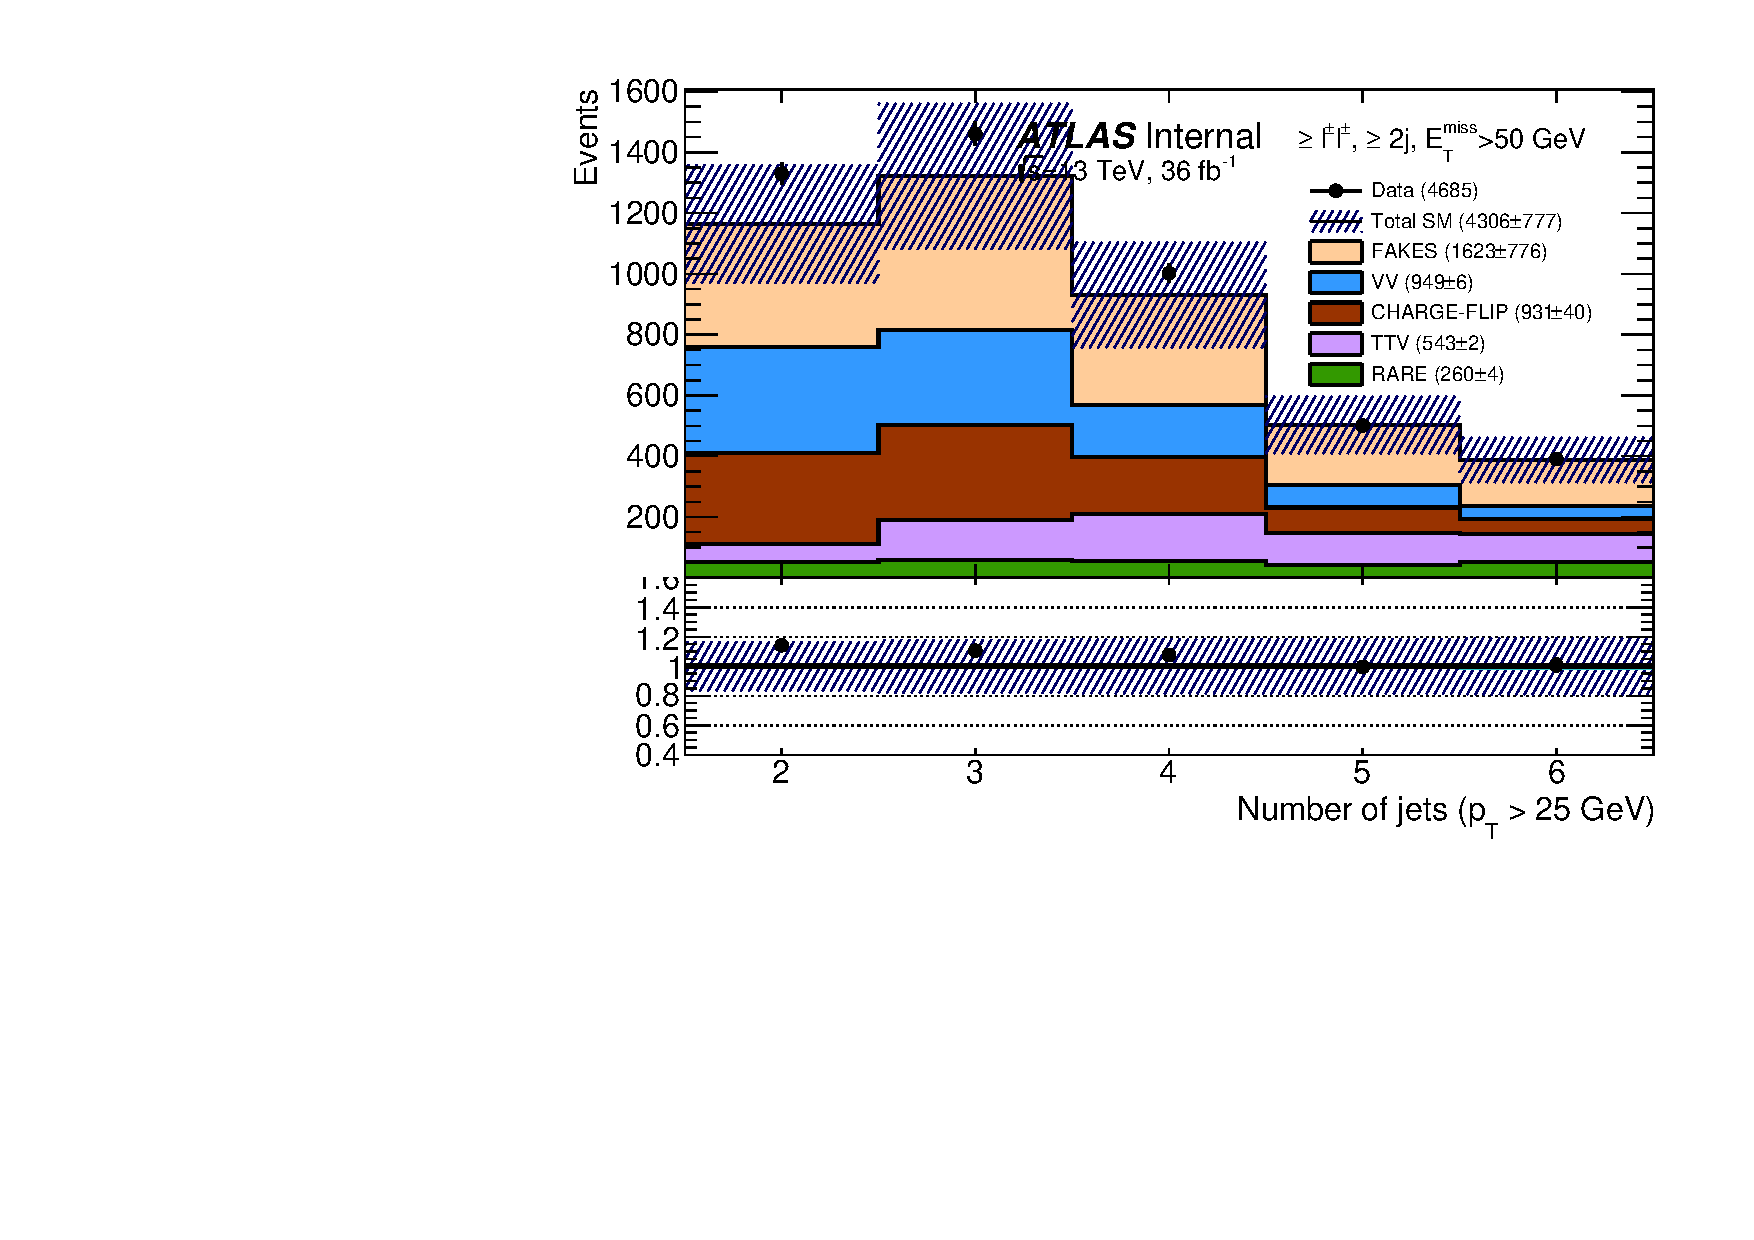
\includegraphics[width=\textwidth]{DILEP_2JMET50_njets25}\caption{}\end{subfigure}
\begin{subfigure}[t]{0.49\textwidth}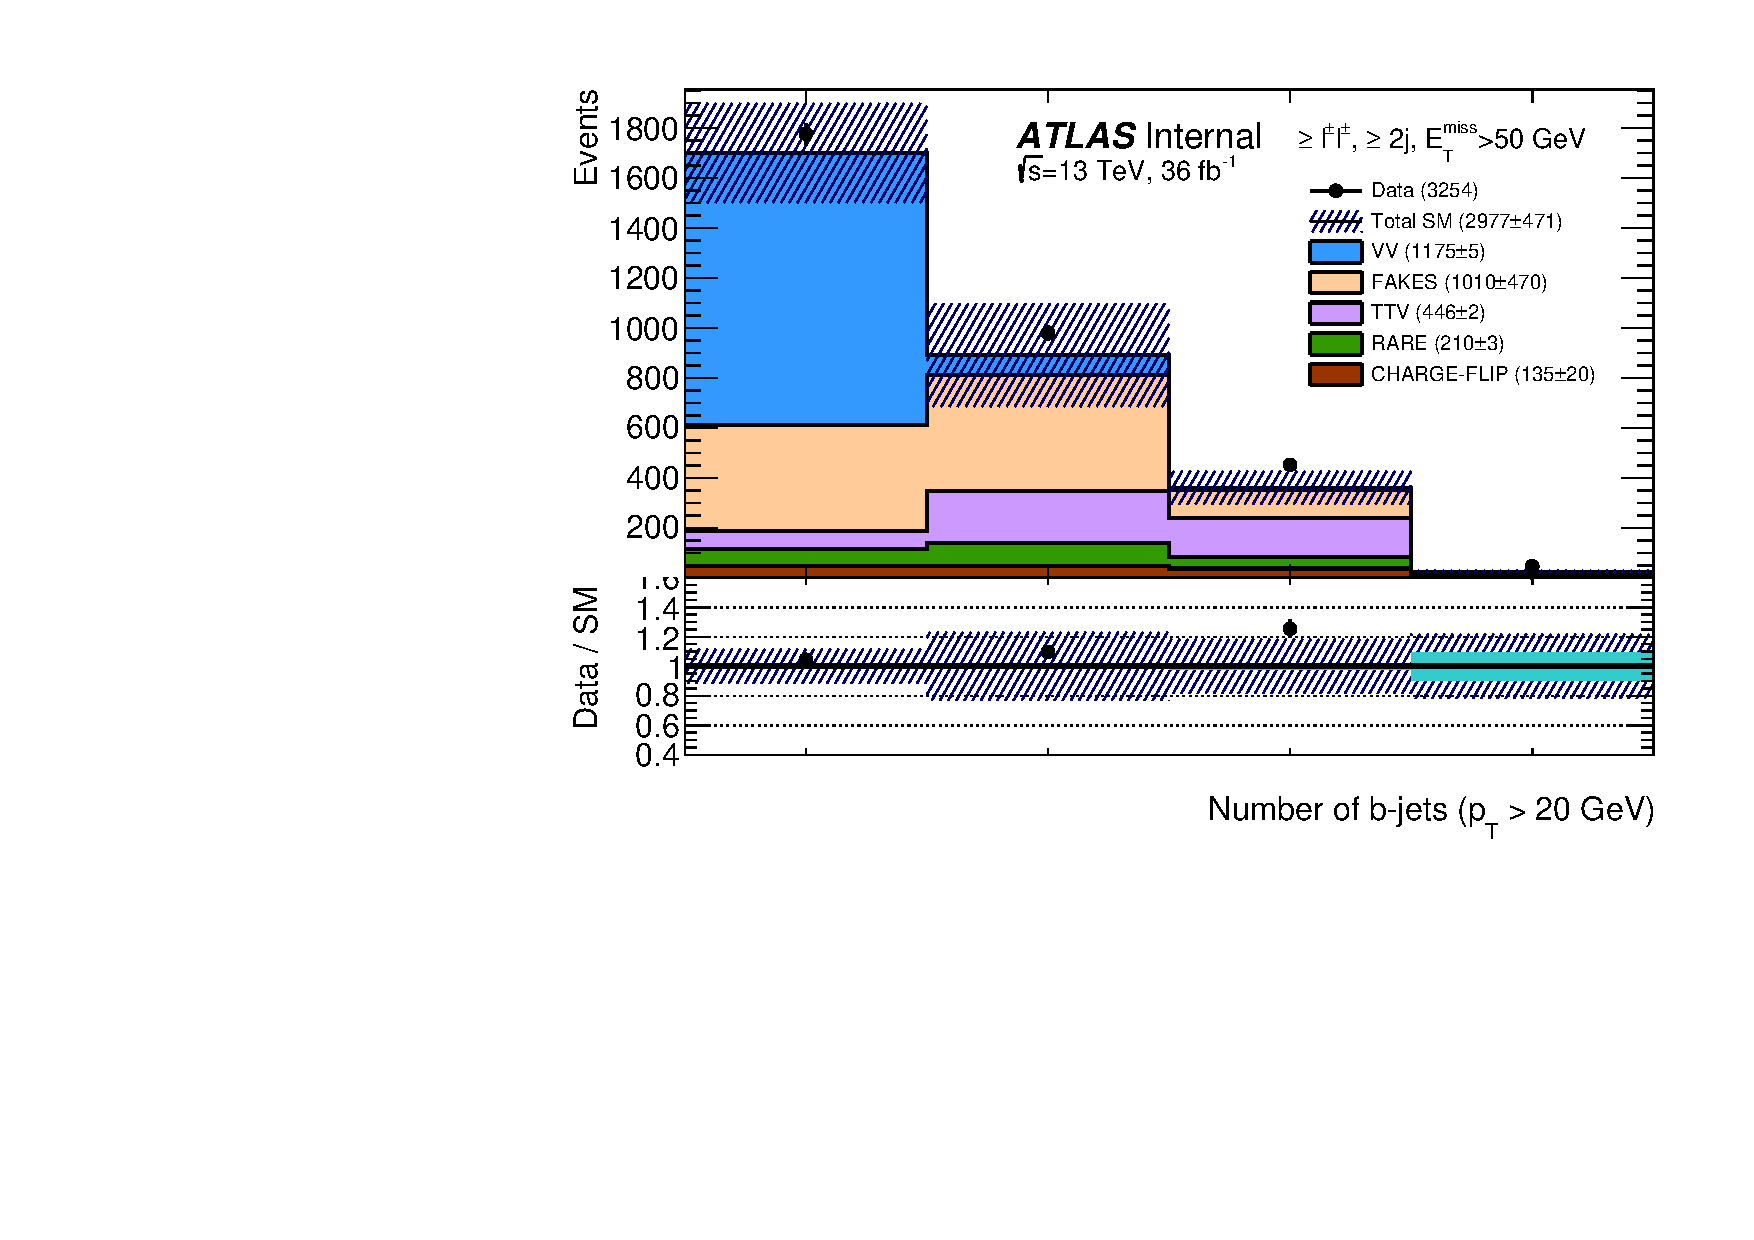
\includegraphics[width=\textwidth]{DILEP_2JMET50_nbjets}\caption{}\end{subfigure}
\begin{subfigure}[t]{0.49\textwidth}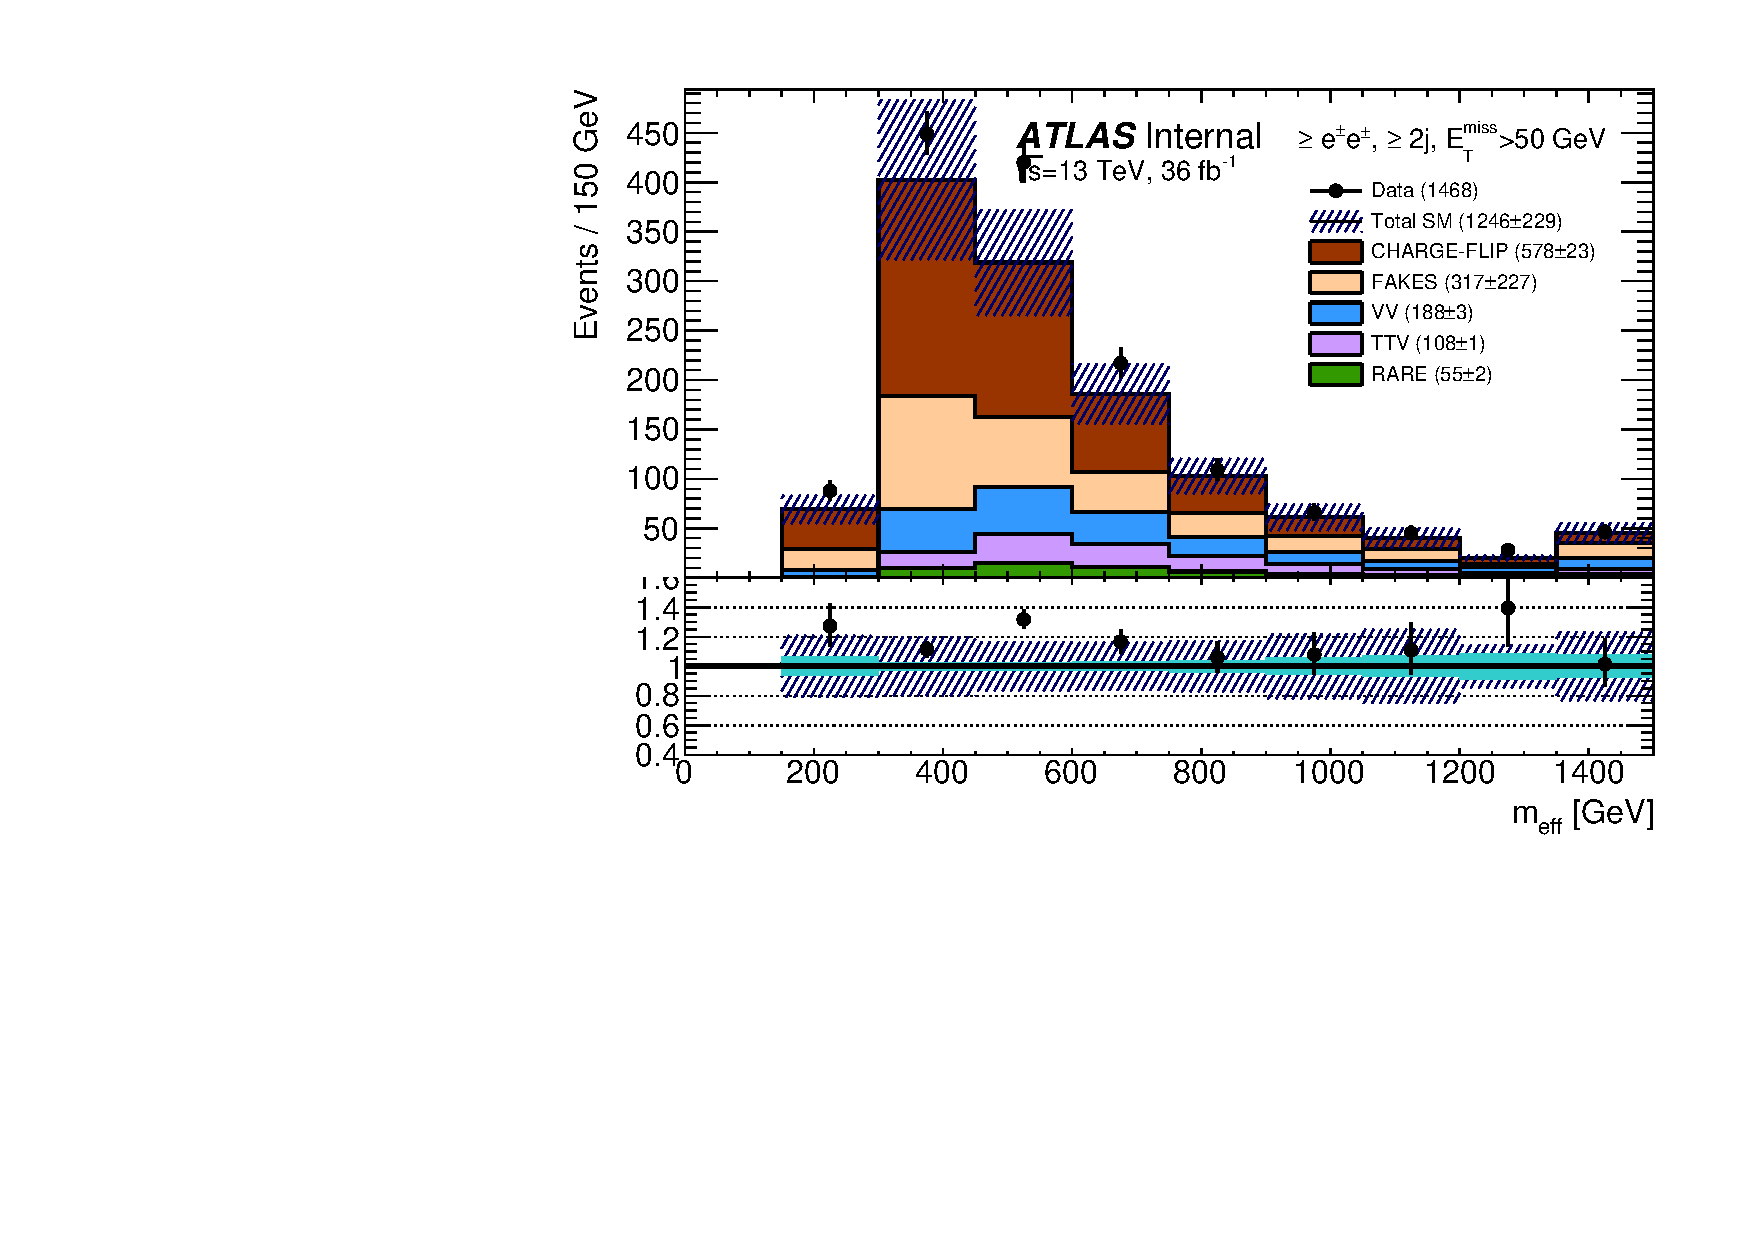
\includegraphics[width=\textwidth]{EE_2JMET50_meff}\caption{}\end{subfigure}
\begin{subfigure}[t]{0.49\textwidth}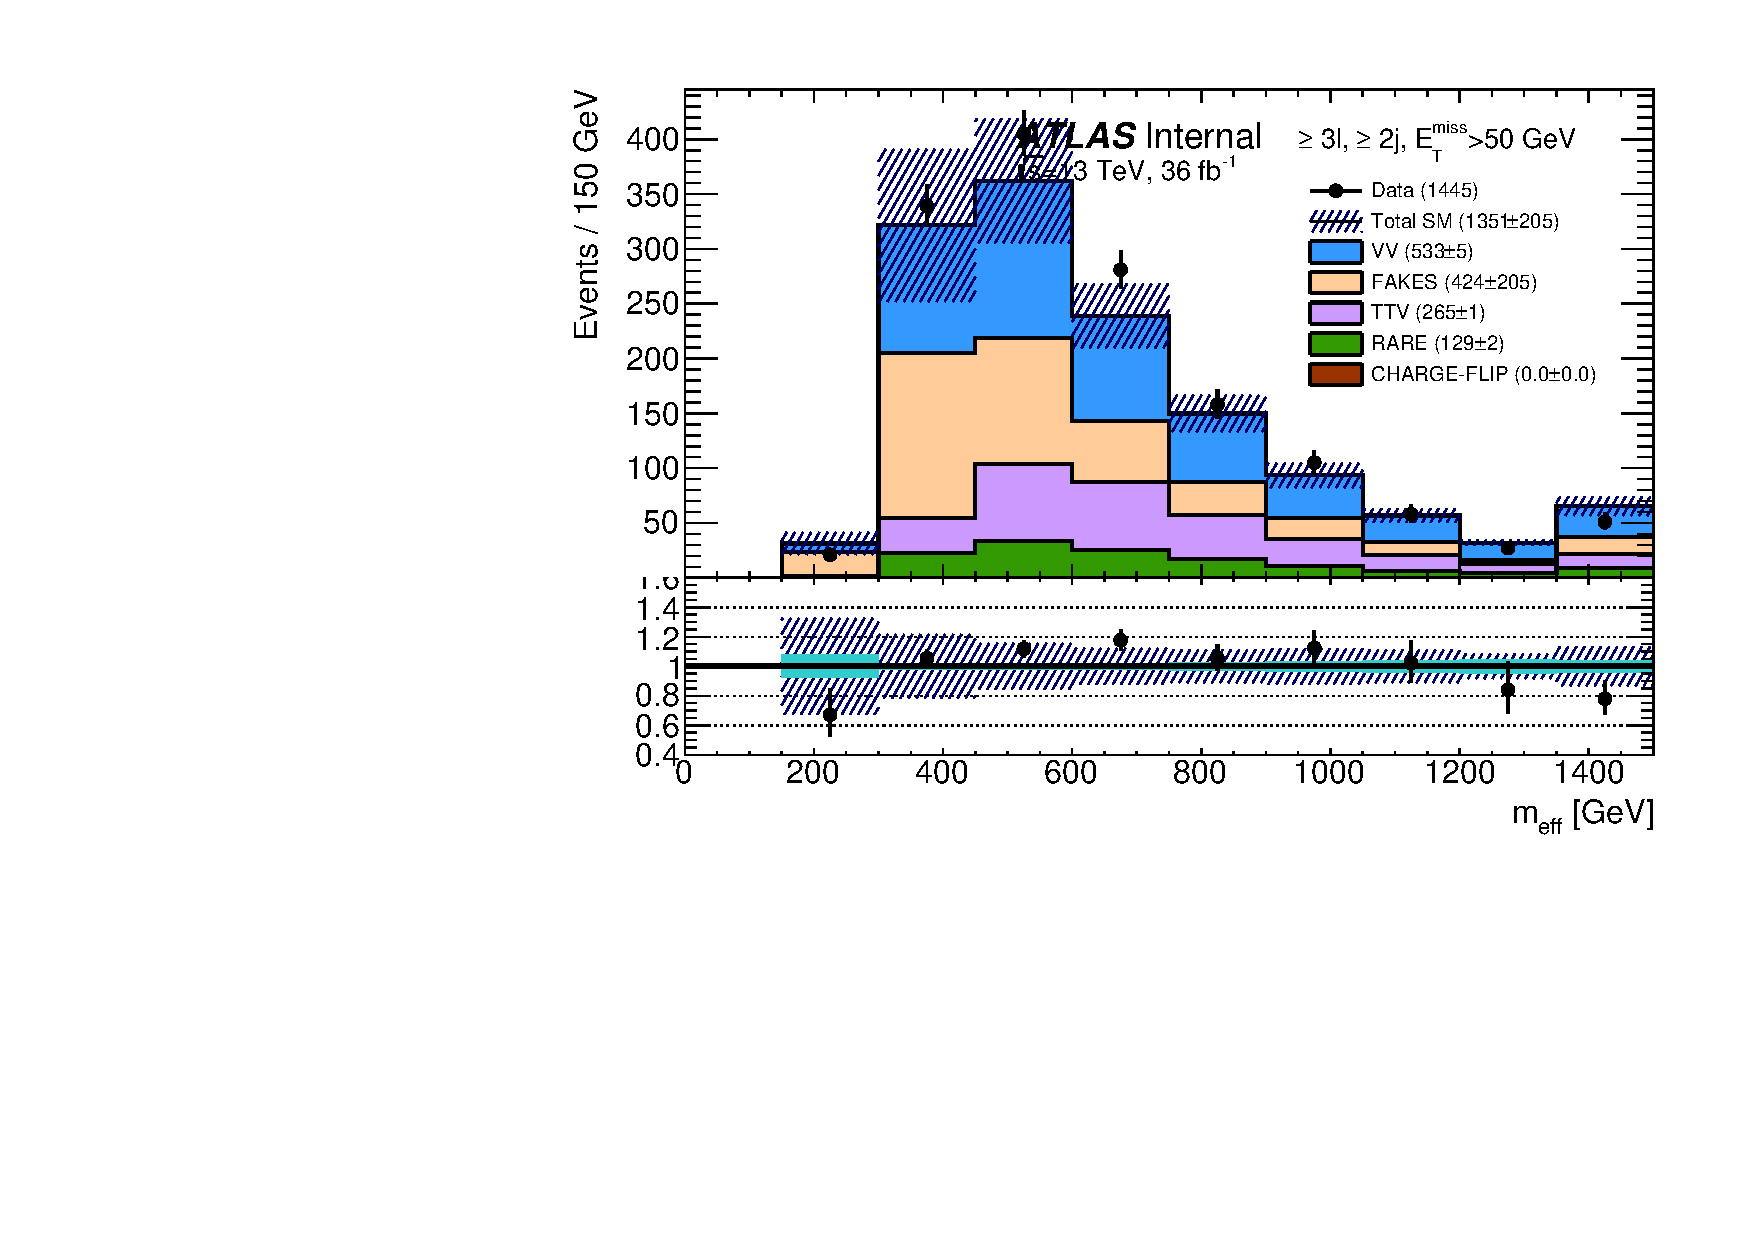
\includegraphics[width=\textwidth]{TRILEP_2JMET50_meff}\caption{}\end{subfigure}
\caption{
Distributions of the number of jets, of $b$-tagged jets and the effective mass after requiring at least two jets ($\pT>\SI{25}{GeV}$) and $\met>\SI{50}{GeV}$, 
as well as at least two same-sign leptons (a,b) or two same-sign electrons (c) or three leptons (d). 
The statistical uncertainties in the background prediction are included in the uncertainty band, 
as well as the full systematic uncertainties for backgrounds with fake or non-prompt leptons, or charge-flip. 
The light blue bands in the ratio plots show contributions from statistical uncertainties alone while the hashed area shows the total uncertainty.. 
The ``Rare'' category contains the contributions from associated production $\ttbar+WW/WZ$, 
as well as $t+Z/WZ/\ttbar$, $H+W/Z$, and triboson production. \textcolor{red}{[UPDATE: Remove numbers in the legend 
and move from upper case to lower case.]}
}
\label{fig:Bkg_distribs} 
\end{figure} 


\subsection{Validation of background estimates}
\label{sec:valid}

To check the validity and robustness of the background estimates, 
the distributions of several discriminating variables in data are compared 
with the predicted background after various requirements on the number of jets and $b$-jets. 
%Events are categorised based on the flavours of the selected leptons, and the different flavour channels are compared separately. 
Examples of such distributions are shown in Fig.~\ref{fig:Bkg_distribs}, 
and illustrate that the predictions and data agree fairly well. 

Dedicated validation regions are defined to test the estimate of the $\ttbar V$, $WZ$ and $W^\pm W^\pm$ SM processes contributing to the signal regions. The corresponding selections are summarized in Table~\ref{tab:VRdef}. 
In these regions, the overlap with the signal regions is resolved by vetoing events that contribute to the signal regions.  
%To further reduce contributions from electron charge mis-identification,  events are also vetoed in VR-$\ttbar W$ and VR-$W^\pm W^{\pm}jj$ if one of the two leading leptons is an electron with $|\eta|>1.37$\textcolor{red}{[UPDATE:Still true]}, since contributions from charge-flip electrons are smaller in the central region due to the lower amount of detector material in front of the calorimeters. 
The purity of the targeted processes in these regions ranges from about \textcolor{red}{[UPDATE:20\% to $50\%$]}. 

The observed yields in these validation regions, compared with the background predictions and uncertainties, 
can be seen in Table~\ref{tab:VR_yields}.
%, and the effective mass distributions are shown in Fig.~\ref{fig:VRd}--\ref{fig:VRf}.
There is good agreement between data and the estimated background for the validation regions.

\begin{table}[t!]
\hspace{0.5cm}
\def\arraystretch{1.1}
\centering
\resizebox{\textwidth}{!}
{\small
\begin{tabular}{|c|c|c|c|c|c|c|l|}
\hline    
Validation        &  $N_{\rm{lepton}}^{\rm{signal}}$ ($N_{\rm{lepton}}^{\rm{cand}}$)   & $N_{b\rm{-jets}}$  &  $N_{\rm{jets}}$  & $p^{}_{\rm{T,jet}}$  & \met\ & \meff\  & Other \\
Region Name       &  &  &  & [GeV]  & [GeV] & [GeV]  & \\
\hline\hline
$W^{\pm} W^{\pm}jj$ & $=2$ ($=2$)    &  $=0$ & $\geq 2$ &   $>50$ & $> 55$  & $> 650$ & veto $81<\mee<101$~GeV  \\
               	  & $=1$ SS pair  &	  &	     &         &   	&	  & $\pt^{\ell_2}>30$~GeV \\
               	  &		  &	  &	     &         &   	&	  & min$\left\{\Delta R(\ell_{1,2},j)\right\}>0.7$ \\
               	  &		  &	  &	     &         &   	&	  & min$\left\{\Delta R(\ell_1, \ell_2)\right\}>1.3$ \\
\hline
$WZ$4j            & $=3$ ($=3$)    &  $=0$ & $\geq 4$ &  $>25$   & --    & $> 450$ & $\met/\sum p_T^{\ell} < 0.7$ \\
\hline
$WZ$5j            & $=3$ ($=3$)    &  $=0$ & $\geq 5$ &  $>25$   & --    & $> 450$ & $\met/\sum p_T^{\ell} < 0.7$  \\ 
\hline
$\ttbar W$   	&$=2$ ($=2$)    &$\geq 1$   & $\geq 4$ ($e^\pm e^\pm$, $e^\pm \mu^\pm$) & $>40$ & $> 45$  & $> 550$   & $\pt(\ell_2)>40$~GeV\\
              	& $=1$ SS pair  &       &  $\geq 3$ ($\mu^\pm \mu^\pm$)   &  $>25$ &      &          & $\sum p_T^{b-jet}/\sum p_T^{jet}>0.25$ \\ 
\hline
$\ttbar Z$    	&$\geq 3$ (-) & $\geq 1$ & $\geq 3$ &  $>35$ &  --    & $> 450$  & $81<m_\text{SFOS}<101$~GeV \\
                &$\geq 1$ SFOS pair&     &          &       &         &         &  \\
\hline
All VRs & \multicolumn{7}{c|}{Veto events belonging to any SR} \\
\hline
\end{tabular}
}
\caption{Summary of the event selection in the validation regions (VRs). 
Requirements are placed on the number of signal leptons ($N_{\rm{lept}}^{\rm{signal}}$) 
and candidate leptons ($N_{\rm{lept}}^{\rm{cand}}$), the number of jets ($N_{\rm{jets}}$) 
or the number of $b$-jets with $\pt>\SI{20}{GeV}$ ($N_{b\rm{-jets}}$). The two leading-\pt 
leptons are referred to as $\ell_{1,2}$ with decreasing \pt. Additional requirements are set 
on \met, \meff, the invariant mass of the two leading electrons $m_{ee}$, the presence of SS 
leptons or a pair of same-flavour opposite-sign leptons (SFOS) and its invariant mass $m_\text{SFOS}$. 
A minimum angular separation between the leptons and the jets ($\Delta R (\ell, j)$) and between the two 
leptons ($\Delta R (\ell_{1}, \ell_2)$) is imposed in $W^\pm W^\pm$ VR. For the two $WZ$ VRs an upper cut 
on the ratio between the \met in the event and the sum of all selected leptons \pt (\met/$\sum{p_T^\ell}$) is required. 
An upper cut on the ratio between the sum of the \pt of all $b$-jets and that of all jets in the event ($\sum p_T^{b-j} / \sum{p_T^{j}}$) is 
considered only in the $\ttbar W$ VR.
}
\label{tab:VRdef}
\end{table}

\begin{table}[t!]
\hspace{0.5cm}
\def\arraystretch{1.1}
\centering
%\resizebox{\textwidth}{!}
%{\small
\begin{tabular}{|l|c|c|c|c|c|}
\hline    
 Validation Regions       & $WZ$4j & $WZ$5j  & $W^\pm W^{\pm}jj$& $\ttbar W$   & $\ttbar Z$  \\
\hline\hline
$t\bar{t}Z/\gamma^*$     & $  \pm  $ & $  \pm  $      & $  \pm  $  & $  \pm  $    & $  \pm  $  \\
$t\bar{t}W$              & $  \pm $  & $  \pm  $      & $  \pm  $  & $  \pm  $    & $  \pm  $  \\
$t\bar{t}H$              & $  \pm $  & $  \pm  $      & $  \pm  $  & $  \pm  $    & $  \pm  $  \\
$t\bar{t}t\bar{t}$       & $  \pm $  & $  \pm  $      & $  \pm  $  & $  \pm  $    & $  \pm  $  \\
$WW$                     & $  \pm $  & $  \pm  $      & $  \pm  $  & $  \pm  $    & $  \pm  $  \\
$WZ$                     & $  \pm $  & $  \pm  $      & $  \pm  $  & $  \pm  $    & $  \pm  $  \\
$ZZ$                     & $  \pm $  & $  \pm  $      & $  \pm  $  & $  \pm  $    & $  \pm  $  \\
Rare                     & $  \pm  $ & $  \pm  $      & $  \pm  $  & $  \pm  $    & $  \pm  $  \\
Fake/non-prompt leptons  & $  \pm  $ & $  \pm  $      & $  \pm  $  & $  \pm  $    & $  \pm $  \\
Charge-flip              & $-$       & $  \pm  $      & $  \pm  $  & $  \pm  $    & $-$  \\
\hline
Total SM  background   	& $-$        & $  \pm  $      & $  \pm  $  & $  \pm  $    & $-$  \\
\hline
Observed	   	& $-$        & $  \pm  $      & $  \pm  $  & $  \pm  $    & $-$  \\
\hline
\end{tabular}
%}
\caption{The numbers of observed data and expected background events in the validation regions. 
The ``Rare'' category contains the contributions from associated production $\ttbar+WW/WZ$, 
as well as $t+Z/WZ/\ttbar$, $H+W/Z$, and triboson production. Background categories shown as a ``$-$'' 
denote that they cannot contribute to a given region (e.g. charge flips in 3-lepton regions). 
The displayed yields include all sources of statistical and systematic uncertainties, 
except for the theoretical uncertainties which only affect the inclusive production cross-sections.}
\label{tab:VR_yields}
\end{table}

\section{Systematic uncertainties on the background estimation}
\label{sec:syst}

Figure~\ref{fig:PlotSR} summarises the contributions of the different sources of systematic uncertainty 
on the total SM background predictions in the signal regions.

The systematic uncertainties related to the same-sign prompt leptons background estimation 
arise from the accuracy of the theoretical and experimental modelling in the MC simulation.
The primary sources of systematic uncertainties are related to the jet energy scale calibration, 
jet energy resolution, $b$-tagging efficiency, and MC modelling and theoretical cross-section uncertainties. 
The statistical uncertainty of the simulated event samples is also taken into account.

The cross-sections used to normalise the MC samples are varied according to the uncertainty in the 
cross-section calculation, that is, 13\% for $\ttbar W$, 12\% for $\ttbar Z$ production~\cite{YR4}, 6\% for diboson
production~\cite{pubnote_mc_multiboson}, 8\% for $\ttbar H$~\cite{YR4} and 30\% for $\ttbar\ttbar$~\cite{Alwall:2014hca}. 
Additional uncertainties are assigned to some of these backgrounds to account for the theoritical modelling of the kinematic 
distributions in the MC simulation. For $\ttbar W$ and $\ttbar Z$, the predictions from the \AMCATNLO and \SHERPA generators are compared, 
and the renormalisation and factorisation scales used to generate these samples are varied, 
leading to a $\sim$\textcolor{red}{[UPDATE:30\%]} uncertainty on the expected SR yields for these processes. 
For dibosons, uncertainties are estimated by varying the renormalisation, factorisation and resummation scales, 
leading to a $\sim$\textcolor{red}{[UPDATE:40-50\%]} uncertainty for these processes after the SR selections. 
For $\ttbar H$, $\ttbar \ttbar$ and Rare production processes, a conservative 50\% uncertainty 
on their total contribution is assigned. 

Uncertainties in the FNP lepton background estimate are assigned due to the limited number 
of data events in the loose and tight lepton control regions.
In addition, systematic uncertainties of \textcolor{red}{[UPDATE:50-60\%]} are assigned to the FNP fake rate to account 
for potentially different 
compositions (heavy flavour, light flavour or conversions) between the regions used to measure these probabilities and the SRs, 
as well as the contamination from prompt leptons in the former regions. Similarly a \textcolor{red}{[UPDATE:5\%]} systematic is assigned to 
$\epsilon$ determination. This leads to overall FNP background uncertainties in the total background estimates 
of \textcolor{red}{[UPDATE:5--32\%]} depending on the signal region.

The uncertainty on the electron charge-flip probability mainly originates from the limited number of events used in 
the charge-flip probability measurement regions and the uncertainty related to the background subtraction 
beyond the $Z$ peak. The relative error on the charge-flip is below \textcolor{red}{[UPDATE:20\%]} for lepton \pt above 20 GeV.

\begin{figure}[H]
\begin{center}
\begin{subfigure}[t]{0.95\textwidth}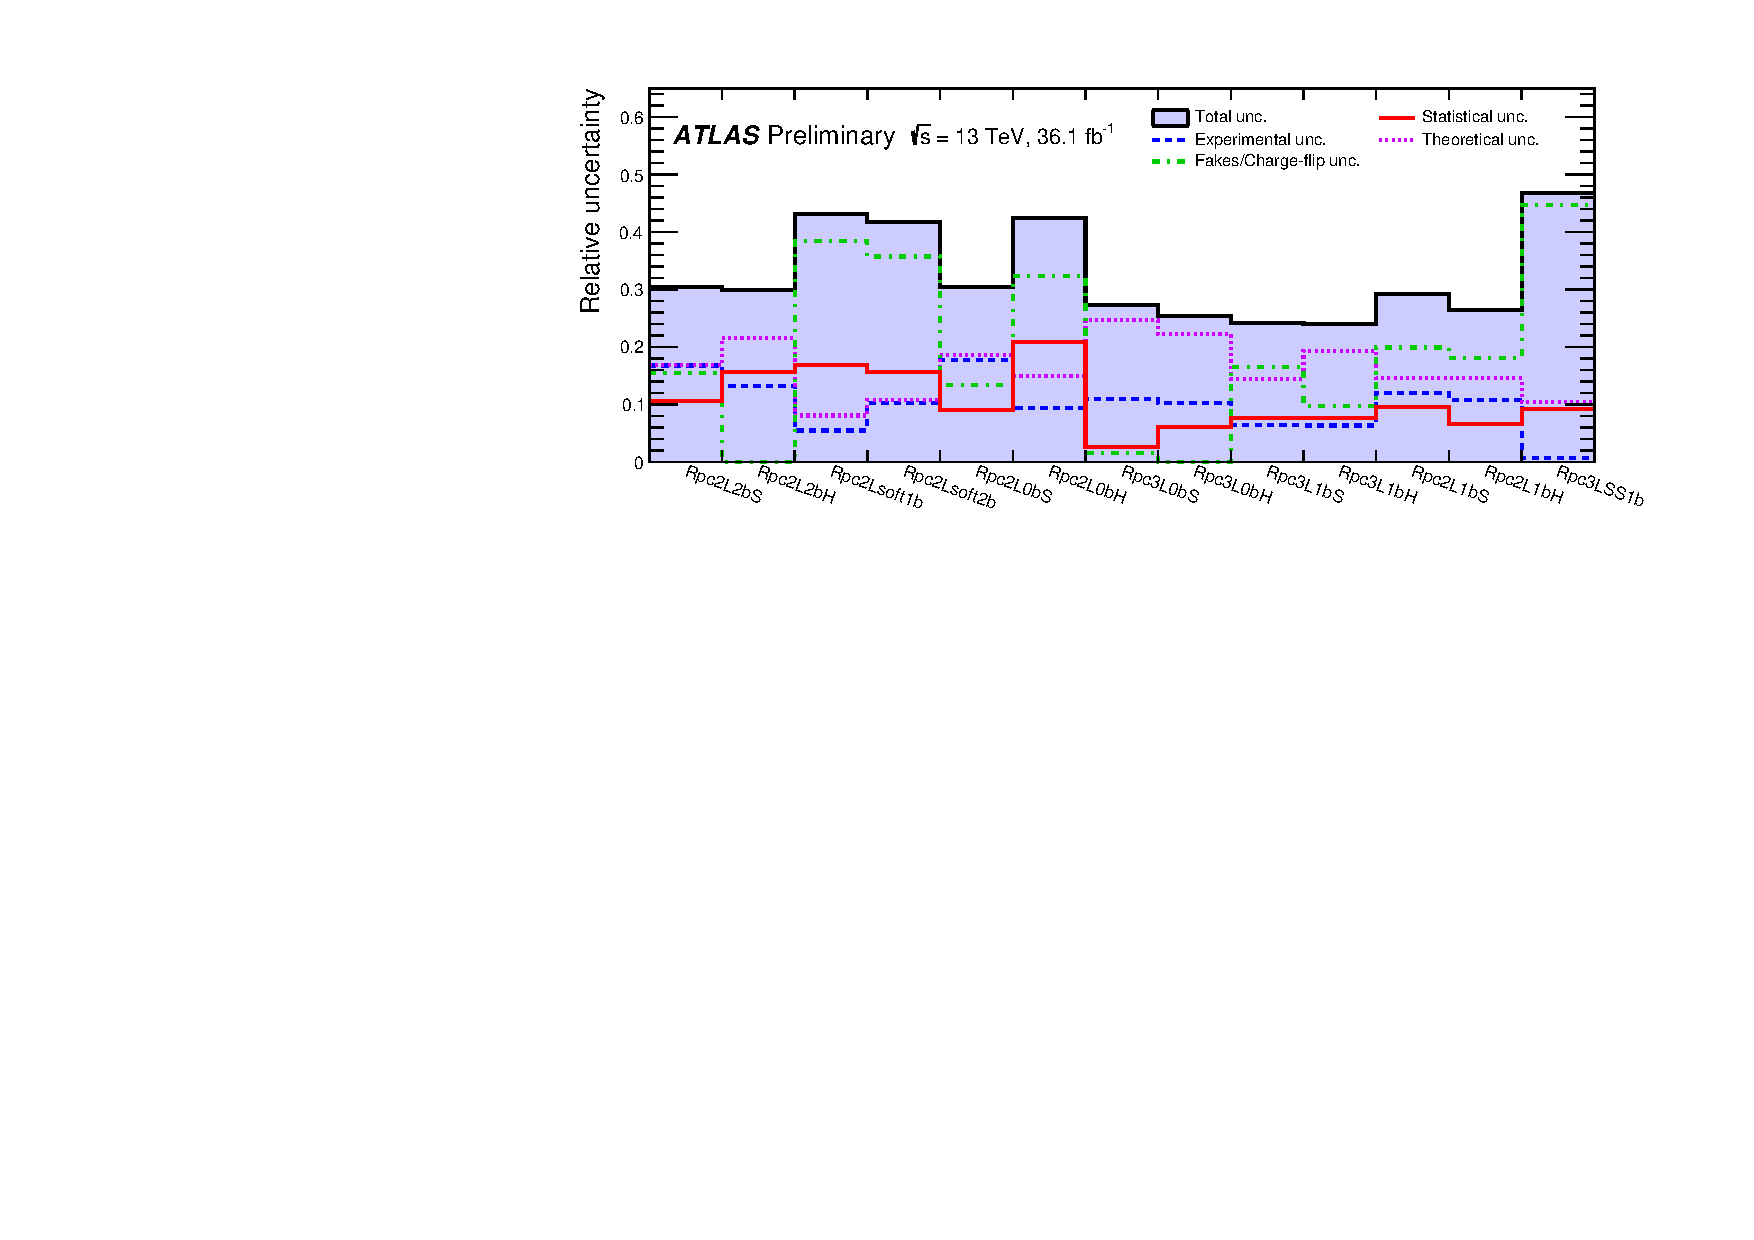
\includegraphics[width=\textwidth]{SystematicsSummary}\caption{}\end{subfigure} \\
\begin{subfigure}[t]{0.87\textwidth}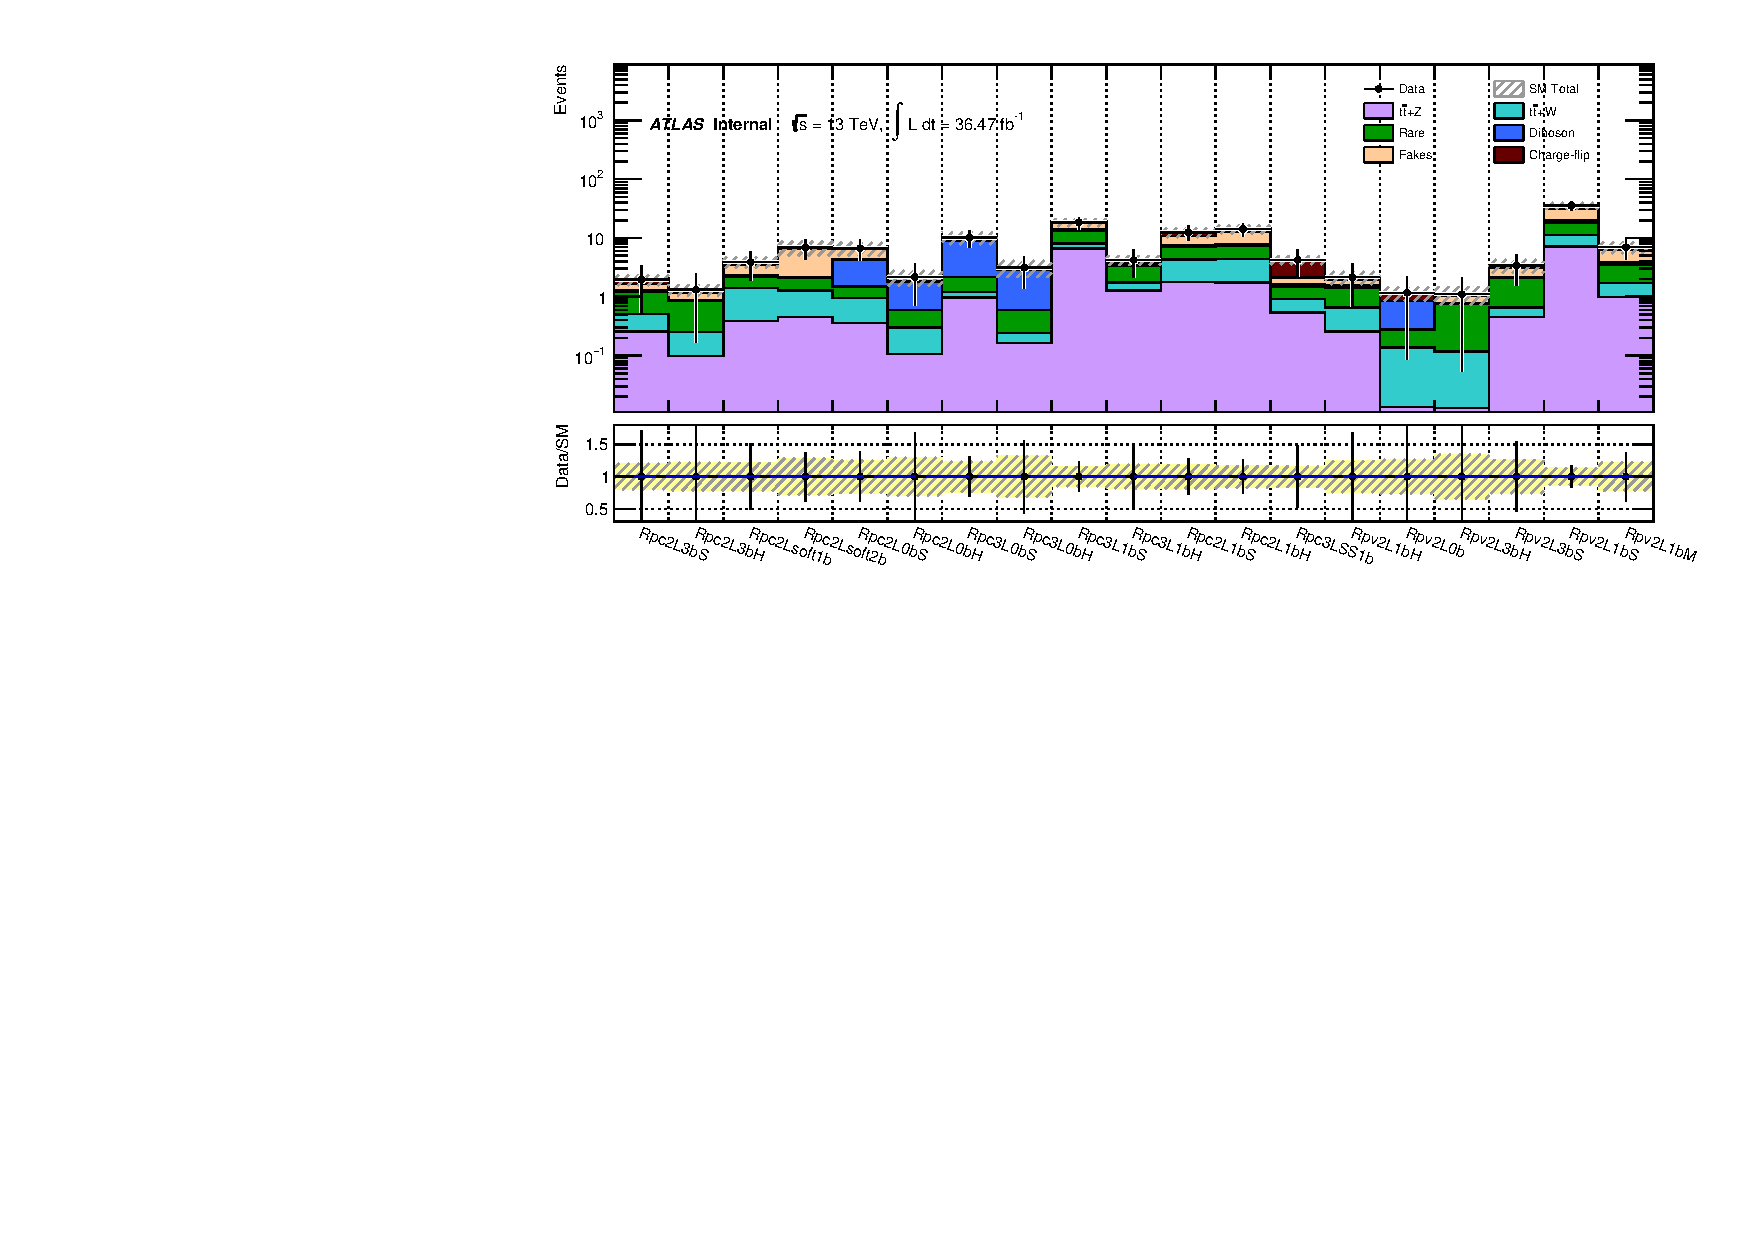
\includegraphics[width=\textwidth]{SRsummary}\caption{}\end{subfigure}
\end{center}
\caption{Relative systematic uncertainties and comparison of the observed and expected event yields in each signal region. 
The background expectations are those obtained from the background-only fits, presented in Table~\ref{tab:SR_yields}. 
\textcolor{red}{[UPDATE: Put all signal regions with final notations. Add ratio plot below SR Event Yields]}} 
\label{fig:PlotSR}
\end{figure}

%\begin{table}[h!]
%\begin{center}
%\caption{The main sources of systematic uncertainty on the SM background estimates for the four signal regions are shown 
%and their values given as relative uncertainties in the expected signal region background event yields. 
%The individual components can be correlated and therefore do not necessarily add up in quadrature to the total systematic uncertainty.
%For reference, the total number of expected background events is also shown.
%}
%\label{tab:SR_syst}
%{\small
%\begin{tabular}{lrrrr}
%\noalign{\smallskip}\hline\hline\noalign{\smallskip}
%         & SR0b3j         & SR0b5j     & SR1b & SR3b     \\[-0.05cm]
%\noalign{\smallskip}\hline\hline\noalign{\smallskip}
%Diboson theoretical uncertainties    & 23\%  &  16\%   &  1\%  &$<$1\%   \\
%$\ttbar V$ theoretical uncertainties & 3\%   &  4\%    & 13\%  &  9\%   \\
%Other theoretical uncertainties      & 5\%   &  3\%    &  9\%  & 15\%   \\
%\noalign{\smallskip}\hline\noalign{\smallskip}
%MC statistical uncertainties         & 11\%  &  14\%   &  3\%  &  6\%   \\
%\noalign{\smallskip}\hline\noalign{\smallskip}
%Jet energy scale        & 12\%   &  11\%  & 6\%    & 5\%   \\
%Jet energy resolution   & 3\%    &  9\%   & 2\%    & 3\%   \\
%$b$-tagging             & 4\%    &  6\%   & 3\%    & 10\%   \\
%PDF                     & 6\%    &  6\%   & 6\%    & 8\%   \\
%Fake/non-prompt leptons & 18\%    &  20\%   & 18\%   & 21\%   \\
%Charge flip             & --     & 1\% & 3\%    & 8\%   \\
%\noalign{\smallskip}\hline\noalign{\smallskip}
%Total background uncertainties & 30\%   & 34\%   & 22\%   & 31\%   \\
%\noalign{\smallskip}\hline\hline\noalign{\smallskip}
%Total background events & $1.5$ & $0.88$ & $4.5$ & $0.80$\\
%\noalign{\smallskip}\hline\hline\noalign{\smallskip}
%\end{tabular}
%}
%\end{center}
%\end{table}
	
